\documentclass[border=6pt]{standalone}
\usepackage{tikz}
\usetikzlibrary{arrows.meta}

\definecolor{birth}{HTML}{009E73}
\definecolor{death}{HTML}{D55E00}

\begin{document}
\pagecolor{white}
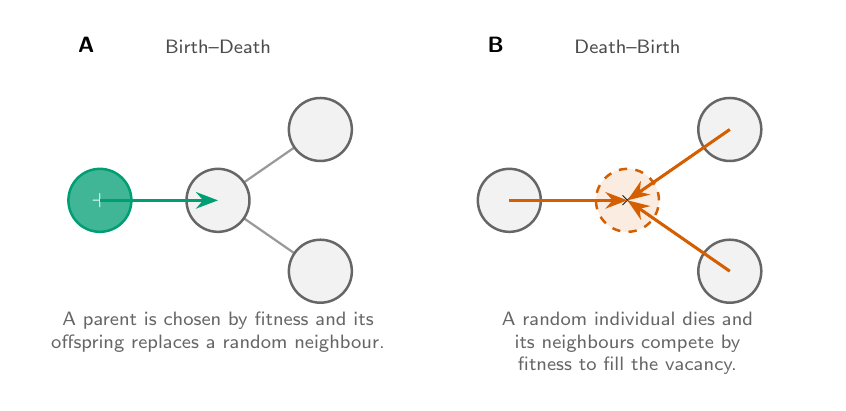
\begin{tikzpicture}[
    font=\sffamily,
    vert/.style={circle, draw=black!60, line width=0.9pt, fill=black!5,
                 minimum size=8mm, inner sep=0pt, font=\sffamily\scriptsize},
    edge/.style={black!40, line width=0.8pt},
    flow/.style={-{Stealth}, line width=1.1pt},
    lab/.style={font=\sffamily\scriptsize, text=black!60, align=center},
    panel/.style={font=\sffamily\footnotesize\bfseries, anchor=north west},
    subcap/.style={font=\sffamily\scriptsize, text=black!70, align=center},
]

% ---- Panel A: Birth-Death ----
\begin{scope}[shift={(0,0)}]
    \node[panel] at (-1.9,2.2) {A};
    \node[subcap] at (0,1.95) {Birth--Death};
    \coordinate (c) at (0,0);
    \coordinate (n1) at (-1.5,0);
    \coordinate (n2) at (1.3,0.9);
    \coordinate (n3) at (1.3,-0.9);
    \draw[edge] (c)--(n1); \draw[edge] (c)--(n2); \draw[edge] (c)--(n3);
    \node[vert] (C) at (c) {};
    \node[vert, fill=birth!75, text=white, draw=birth] (N1) at (n1) {$+$};
    \node[vert] (N2) at (n2) {};
    \node[vert] (N3) at (n3) {};
    \draw[flow, birth] (n1) -- (c);
    \node[lab, anchor=north, text width=4.6cm] at (0,-1.3)
        {A parent is chosen by fitness and its offspring replaces a random
         neighbour.};
\end{scope}

% ---- Panel B: Death-Birth ----
\begin{scope}[shift={(5.2,0)}]
    \node[panel] at (-1.9,2.2) {B};
    \node[subcap] at (0,1.95) {Death--Birth};
    \coordinate (c) at (0,0);
    \coordinate (n1) at (-1.5,0);
    \coordinate (n2) at (1.3,0.9);
    \coordinate (n3) at (1.3,-0.9);
    \draw[edge] (c)--(n1); \draw[edge] (c)--(n2); \draw[edge] (c)--(n3);
    \node[vert, draw=death, dashed, fill=death!12] (C) at (c) {$\times$};
    \node[vert] (N1) at (n1) {};
    \node[vert] (N2) at (n2) {};
    \node[vert] (N3) at (n3) {};
    \draw[flow, death] (n1) -- (c);
    \draw[flow, death] (n2) -- (c);
    \draw[flow, death] (n3) -- (c);
    \node[lab, anchor=north, text width=4.6cm] at (0,-1.3)
        {A random individual dies and its neighbours compete by fitness to
         fill the vacancy.};
\end{scope}
\end{tikzpicture}
\end{document}
